% This is "sig-alternate.tex" V1.9 April 2009
% This file should be compiled with V2.4 of "sig-alternate.cls" April 2009
%
% This example file demonstrates the use of the 'sig-alternate.cls'
% V2.4 LaTeX2e document class file. It is for those submitting
% articles to ACM Conference Proceedings WHO DO NOT WISH TO
% STRICTLY ADHERE TO THE SIGS (PUBS-BOARD-ENDORSED) STYLE.
% The 'sig-alternate.cls' file will produce a similar-looking,
% albeit, 'tighter' paper resulting in, invariably, fewer pages.
%
% ----------------------------------------------------------------------------------------------------------------
% This .tex file (and associated .cls V2.4) produces:
%       1) The Permission Statement
%       2) The Conference (location) Info information
%       3) The Copyright Line with ACM data
%       4) NO page numbers
%
% as against the acm_proc_article-sp.cls file which
% DOES NOT produce 1) thru' 3) above.
%
% Using 'sig-alternate.cls' you have control, however, from within
% the source .tex file, over both the CopyrightYear
% (defaulted to 200X) and the ACM Copyright Data
% (defaulted to X-XXXXX-XX-X/XX/XX).
% e.g.
% \CopyrightYear{2007} will cause 2007 to appear in the copyright line.
% \crdata{0-12345-67-8/90/12} will cause 0-12345-67-8/90/12 to appear in the copyright line.
%
% ---------------------------------------------------------------------------------------------------------------
% This .tex source is an example which *does* use
% the .bib file (from which the .bbl file % is produced).
% REMEMBER HOWEVER: After having produced the .bbl file,
% and prior to final submission, you *NEED* to 'insert'
% your .bbl file into your source .tex file so as to provide
% ONE 'self-contained' source file.
%
% ================= IF YOU HAVE QUESTIONS =======================
% Questions regarding the SIGS styles, SIGS policies and
% procedures, Conferences etc. should be sent to
% Adrienne Griscti (griscti@acm.org)
%
% Technical questions _only_ to
% Gerald Murray (murray@hq.acm.org)
% ===============================================================
%
% For tracking purposes - this is V1.9 - April 2009

\documentclass{sig-alternate}

\begin{document}
%
% --- Author Metadata here ---
%\conferenceinfo{WOODSTOCK}{'97 El Paso, Texas USA}
%\CopyrightYear{2007} % Allows default copyright year (200X) to be over-ridden - IF NEED BE.
%\crdata{0-12345-67-8/90/01}  % Allows default copyright data (0-89791-88-6/97/05) to be over-ridden - IF NEED BE.
% --- End of Author Metadata ---

\title{General Theories of Software Defect Prediction: A Preliminary Report}
%\subtitle{[Extended Abstract]
\titlenote{A full version of this paper is available as
\textit{Author's Guide to Preparing ACM SIG Proceedings Using
\LaTeX$2_\epsilon$\ and BibTeX} at
\texttt{www.acm.org/eaddress.htm}}}
%
% You need the command \numberofauthors to handle the 'placement
% and alignment' of the authors beneath the title.
%
% For aesthetic reasons, we recommend 'three authors at a time'
% i.e. three 'name/affiliation blocks' be placed beneath the title.
%
% NOTE: You are NOT restricted in how many 'rows' of
% "name/affiliations" may appear. We just ask that you restrict
% the number of 'columns' to three.
%
% Because of the available 'opening page real-estate'
% we ask you to refrain from putting more than six authors
% (two rows with three columns) beneath the article title.
% More than six makes the first-page appear very cluttered indeed.
%
% Use the \alignauthor commands to handle the names
% and affiliations for an 'aesthetic maximum' of six authors.
% Add names, affiliations, addresses for
% the seventh etc. author(s) as the argument for the
% \additionalauthors command.
% These 'additional authors' will be output/set for you
% without further effort on your part as the last section in
% the body of your article BEFORE References or any Appendices.

\numberofauthors{3} %  in this sample file, there are a *total*
% of EIGHT authors. SIX appear on the 'first-page' (for formatting
% reasons) and the remaining two appear in the \additionalauthors section.
%
\author{
% You can go ahead and credit any number of authors here,
% e.g. one 'row of three' or two rows (consisting of one row of three
% and a second row of one, two or three).
%
% The command \alignauthor (no curly braces needed) should
% precede each author name, affiliation/snail-mail address and
% e-mail address. Additionally, tag each line of
% affiliation/address with \affaddr, and tag the
% e-mail address with \email.
%
% 1st. author
\alignauthor
William Mensah\\
       \affaddr{WVU, Morgantown, WV}\\
       \email{wmensah@csee.wvu.edu}
% 2nd. author
\alignauthor
Adam Nelson\\
       \affaddr{WVU, Morgantown, WV}\\
       \email{anelson8@csee.wvu.edu}
% 3rd. author
\alignauthor 
Tomi Prifti\\
       \affaddr{WVU, Morgantown, WV}\\
       \email{tprifi@csee.wvu.edu}
%\and  % use '\and' if you need 'another row' of author names
% 4th. author
%\alignauthor Lawrence P. Leipuner\\
%       \affaddr{Brookhaven Laboratories}\\
%       \affaddr{Brookhaven National Lab}\\
%       \affaddr{P.O. Box 5000}\\
%       \email{lleipuner@researchlabs.org}
% 5th. author
%\alignauthor Sean Fogarty\\
%       \affaddr{NASA Ames Research Center}\\
%       \affaddr{Moffett Field}\\
%       \affaddr{California 94035}\\
%       \email{fogartys@amesres.org}
% 6th. author
%\alignauthor Charles Palmer\\
%       \affaddr{Palmer Research Laboratories}\\
%       \affaddr{8600 Datapoint Drive}\\
%       \affaddr{San Antonio, Texas 78229}\\
%       \email{cpalmer@prl.com}
}
% There's nothing stopping you putting the seventh, eighth, etc.
% author on the opening page (as the 'third row') but we ask,
% for aesthetic reasons that you place these 'additional authors'
% in the \additional authors block, viz.
%\additionalauthors{Additional authors: John Smith (The Th{\o}rv{\"a}ld Group,
%email: {\texttt{jsmith@affiliation.org}}) and Julius P.~Kumquat
%(The Kumquat Consortium, email: {\texttt{jpkumquat@consortium.net}}).}
\date{30 July 1999}
% Just remember to make sure that the TOTAL number of authors
% is the number that will appear on the first page PLUS the
% number that will appear in the \additionalauthors section.

\maketitle
\begin{abstract}
This paper provides a sample of a \LaTeX\ document which conforms,
somewhat loosely, to the formatting guidelines for
ACM SIG Proceedings. It is an {\em alternate} style which produces
a {\em tighter-looking} paper and was designed in response to
concerns expressed, by authors, over page-budgets.
It complements the document \textit{Author's (Alternate) Guide to
Preparing ACM SIG Proceedings Using \LaTeX$2_\epsilon$\ and Bib\TeX}.
This source file has been written with the intention of being
compiled under \LaTeX$2_\epsilon$\ and BibTeX.

The developers have tried to include every imaginable sort
of ``bells and whistles", such as a subtitle, footnotes on
title, subtitle and authors, as well as in the text, and
every optional component (e.g. Acknowledgments, Additional
Authors, Appendices), not to mention examples of
equations, theorems, tables and figures.

To make best use of this sample document, run it through \LaTeX\
and BibTeX, and compare this source code with the printed
output produced by the dvi file. A compiled PDF version
is available on the web page to help you with the
`look and feel'.
\end{abstract}

% A category with the (minimum) three required fields
\category{H.4}{Information Systems Applications}{Miscellaneous}
%A category including the fourth, optional field follows...
\category{D.2.8}{Software Engineering}{Metrics}[complexity measures, performance measures]

\terms{Delphi theory}

\keywords{ACM proceedings, \LaTeX, text tagging}

\section{Introduction} 
By predicting defects in software systems {\em before} the deployment of that software, 
it is possible to gauge not only the probable quality upon delivery, but also the maintenance effort. 
Software defect prediction builds models using available company data that can then be applied in order 
to predict these software faults. But in order to employ these models, a company must have 
a data repository where information regarding defects from past projects are stored. 
However, according to Turhan, et. al. \cite{turhan09}, few companies are applying this practice. 
Turhan, et. al. claims (and we agree), that this is most likely due to a lack of local data repositories.
When this is the case, companies must use non-local data in order to build defect predictors. Thus, 
it is not only important to determine how well cross-company data can be used when local data is unavailable, 
but also to find the presence or absence of a general theory of software defect prediction. In other words, 
in determining the existence of an empirically-derived correlation between varying defect data sets, 
a statement can be made in regards to not only the stability of current defect prediction, but also the 
underlying similarities of cross-company software projects. On the other hand, 
if no correlation is found to exist, instability of those current predictors may suggest that further research 
should be conducted in order to provide incite into the variance between projects. 

%In this paper, we provide introduce recent experiments conducted by the authors of this paper in order to produce 
%a general hypothesis in regards to the stability or instability of current software defect prediction theories that can be used in further analyses.   

\section{Background}

The ability of an organization being able to use cross-company (CC) data 
when within-company (WC) data is not available in order to build 
defect predictors would be advantageous. However, it remains unclear 
if this practice can yield beneficial results.  
	
Turhan et al. conducted three experiments to rule in favor of CC data obtained from other sites, or WC data gathered locally. The conclusions of those experiments show that CC data, when applied using {\em relevancy filtering} via a k-nearest neighbor scheme. The idea behind the k-NN filter is simple; by building a training set that is homogeneous with the testing set, it is assumed that a bias in the model will be introduced. The filter works as follows: for each instance in the test set, the k nearest neighbors in the training set are chosen. Then, duplicates are removed and the remaining instances are used as the new training set. This relevancy filtering can lead to defect predictors almost as effective as WC data. Thus, as stated by Gay et. al. \cite{gay09}, ``...while local data is the preferred option, it is feasible to use imported data provided that it is selected by a relevancy filter.''

Gat et. al. confirmed Turhan et. al.'s results, but instead of implementing a nearest neighbor filter, a locally weighted scheme was used to filter the data via \cite{hallLWL}. This experiment was of significance due to the fact that Gay et. al.'s results showed not only that CC data can be used when local data is not available, but also that publicly available data such as the PROMISE \footnote{http://promisedata.org/} data.

On the other hand, \cite{zimmerman09} shows that CC data cannot be used to build accurate defect predictors. For example, in one experiment conducted by Zimmerman et. al., Firefox and Internet Explorer were used due to their domain relationship (browsers) in order to determine how well one could predict for the other. It was found that while Firefox could predict for Internet Explorer at a precision of 76.47\%, Firefox could {\em not} predict for Internet Explorer approaching the same precision (4.12\%). However, this experiment did not utilize any form of relevancy filtering, so it is unknown how the two data sets would react to predicting for one another under these circumstances. 

If CC data, when filtered, can be used in order to predict defects, we are left to assume that this is due to the fact that the data sets share some innate similarities of their metrics. But if it is found conclusively that CC data cannot most generally build good defect predictors, we are to conclude that other measures must be taken in either the collection of the WC data, or for more research in the further filtering of CC data.

\subsection{Defect Prediction Stability}



\section{The Experiment}

\subsection{Preparing the Data}
We employed a number of preprocessing techniques to prepare the original data before applying our learner to it. These include:

\begin{itemize}
\item{Logging}
\\Replacing all number values N with log(N) when N > 0.0001 or with 0.0001 if otherwise.
\item{Binning}
\\Splitting each data set into {\em 10} bins (by default) and then building train data from 90\% of the data and 10\% from what is left.
\item{Clustering}
\\Partitioning {\em n} observations from each data set into k clusters using {\em k-means} algorithm whereby each observation belongs to the cluster with the nearest mean.
\item{Feature Subset Selection}
\\Sample bias via {\em InfoGain} whereby each column in the data set is ranked by some criteria and the top n columns are maintained and used for the experiment because they are more likely to have a stronger influence on the results.
\end{itemize}
Why are all these preprocessing techniques necessary and why is time wasted them before the learner is applied? Why not use the data in its raw form? When it comes to data mining, real world data is considered by most software engineers as {\em dirty}. This is because the data could be incomplete, that is, be missing some attributes or attribute values or it could simply consist of only aggregated values. In addition to that, the data could be inconsistent, and could also contain errors and outliers.


\subsection{Discretization techniques}
Two discretization method were used for performing the experiments: Equal Interval Width (10 bins) and K-Means. Both methods fall under the unsupervized discretization methods class. Equal bin length is a global techinque which replaces each value by the identifier of the bin. The range of values is divided into k equally sized bins where k is a parameter supplied by the user. It makes no use of the instance class and is thus an unsupervized discretization method. Equal Bin Length is a global discretization  method since it produces a mesh over the entire n-dimensional instance space \cite {dough95}. The k-means on the other hand is a local discretization tool which groups the data into a number of clusters based on some similarity measure. Local discretization methods are applied to local regions of the data.K-Means is grouping the rows in k different clusters using the Eucledian distance as a measure of similarity between the instances. At the beginning the centroids (means) for each cluster are picked at random and then the instances are assigned to the group with the closest centroids to that particular instance. K-Means will stop iteration through the instance set when the centroids for all the clusters do not change anymore or when a stopping criteria is reached. In both cases of discretization the data is preprocessed by taking the log of each numeric value. Since these two method do not take into consideration class lables there might be some loss of classification information as a result of grouping instances that are stronly related but belong to different classes. 
Since our main learning algorithm is Naive-Bayes, both discretization method greatly improve the performance of the learner. Naive-Bayes is used with both k-means clustering and equal interval width bins on each of the datasets.

\section{Results}
Naive-Bayes learner was applied on all data sets. Three learners were tested
\begin{itemize}
\item{Naive-Bayes without discretizing. K-means applied on the data}
\\In this experiment the data was supplied to the learner without performing any discretization. After splitting the data the train set was clustered using k-means. For each instance on the test data set the closest cluster was determined and the instance was classified using Naive-Bayes trained on that specific cluster.The performance of the learner was tested on different number of clusters k ranging from 2 to 7
\item{Naive-Bayes with  discretization (10 bins). InfoGain applied on the data}
\\After discretizing the data InfoGain was applied on the whole data set to retrieve n number of features (columns) where n is a user specified value ranging from 2 to 14.   
\item{Filter the features with InfoGain. Apply Naive-Bayes with clustering}
\\In this experiment InfoGain was applied to select the n best features. After selecting the best features a new dataset was build out of the original dataset containing only the selected features returned by InfoGain. The new dataset is clustered using K-Means. The learner is tested using different combinations of n-number of features and k-number of clusters
\end{itemize}

Running the first learner, Naive-Bayes without discretization on different datasets shows clearly that discretiztion effect the performance of Naive-Byaes. Figure 1 and 2 show the PD PF values after running the learner with different k number of clusters.
\textbf
\begin
  \begin{center}
    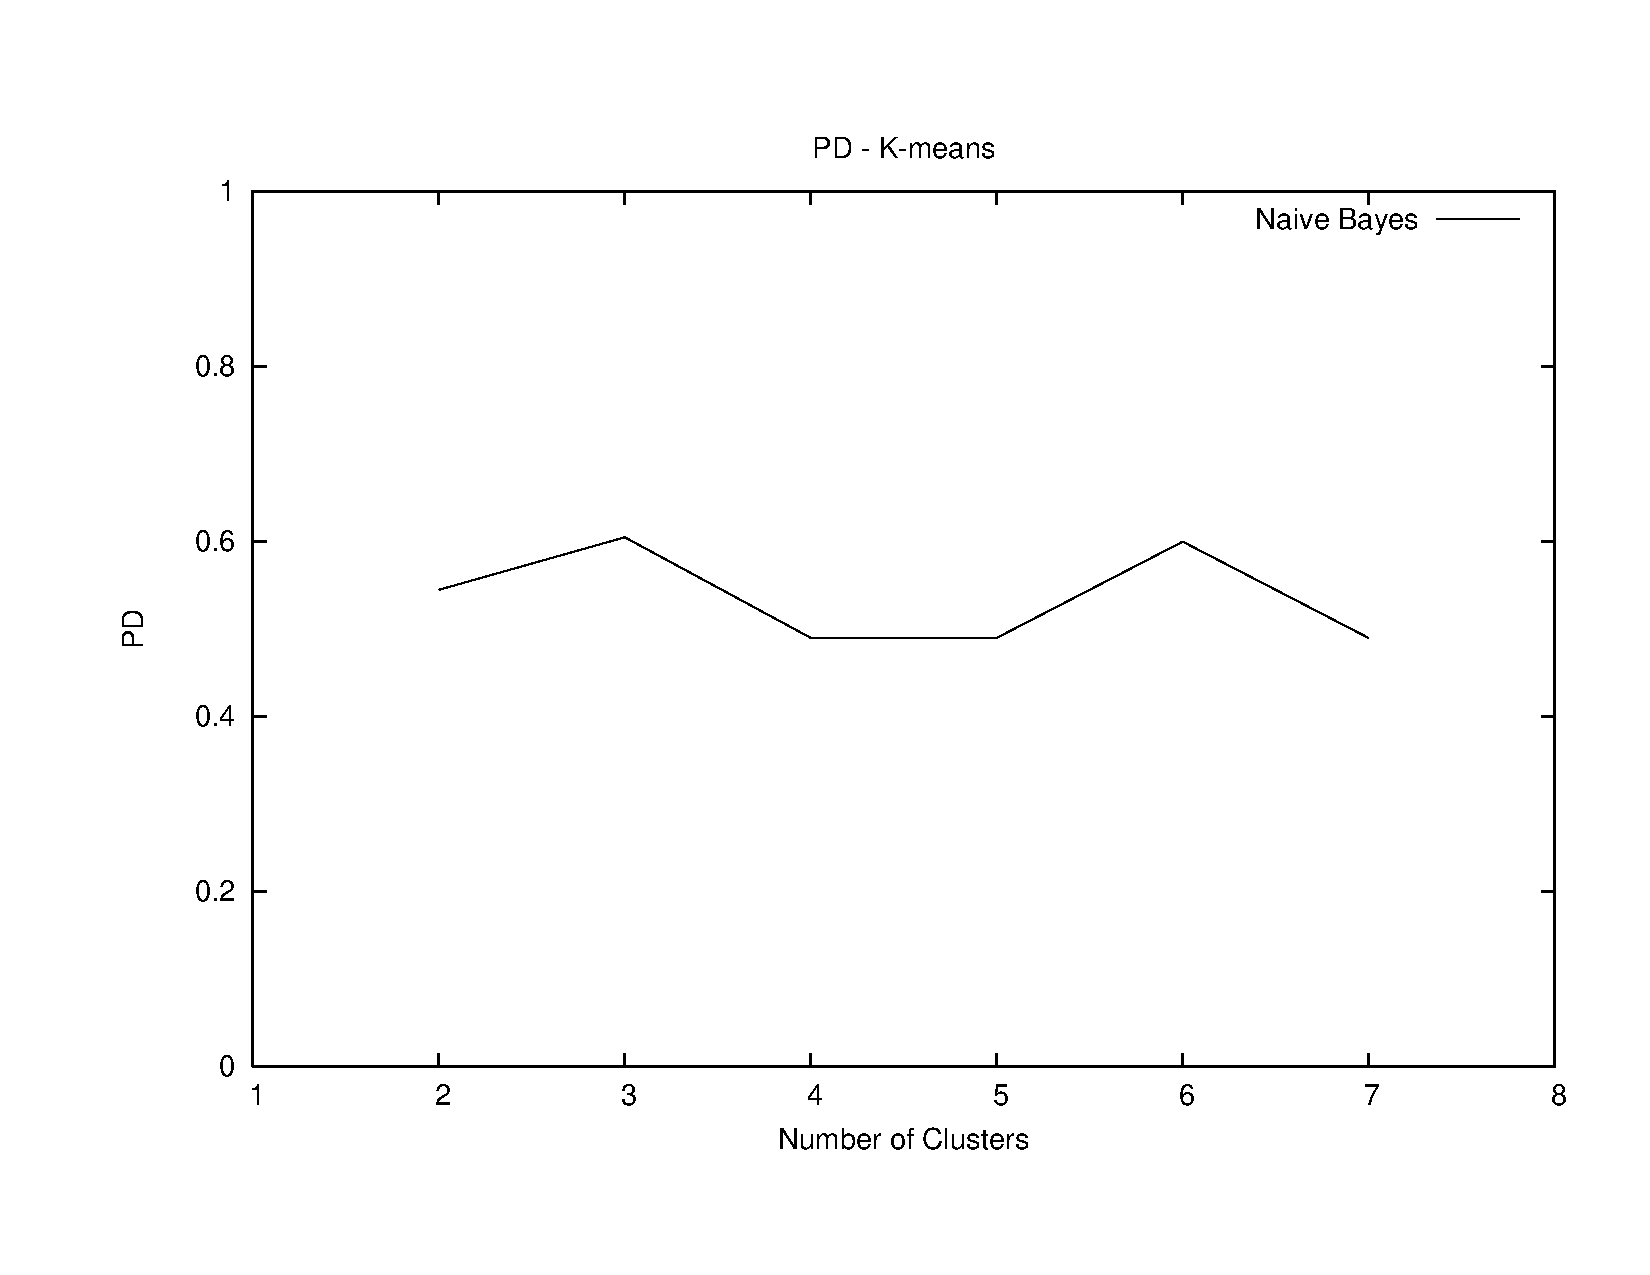
\includegraphics[width=3.5in]{no_disc_nb_cluster_pd.pdf}
  \end{center}

  \caption{\small Figure 1. PD: Naive-Bayes without discretization}
  \label{fig-label}
\end{figure}

\textbf
\begin
  \begin{center}
    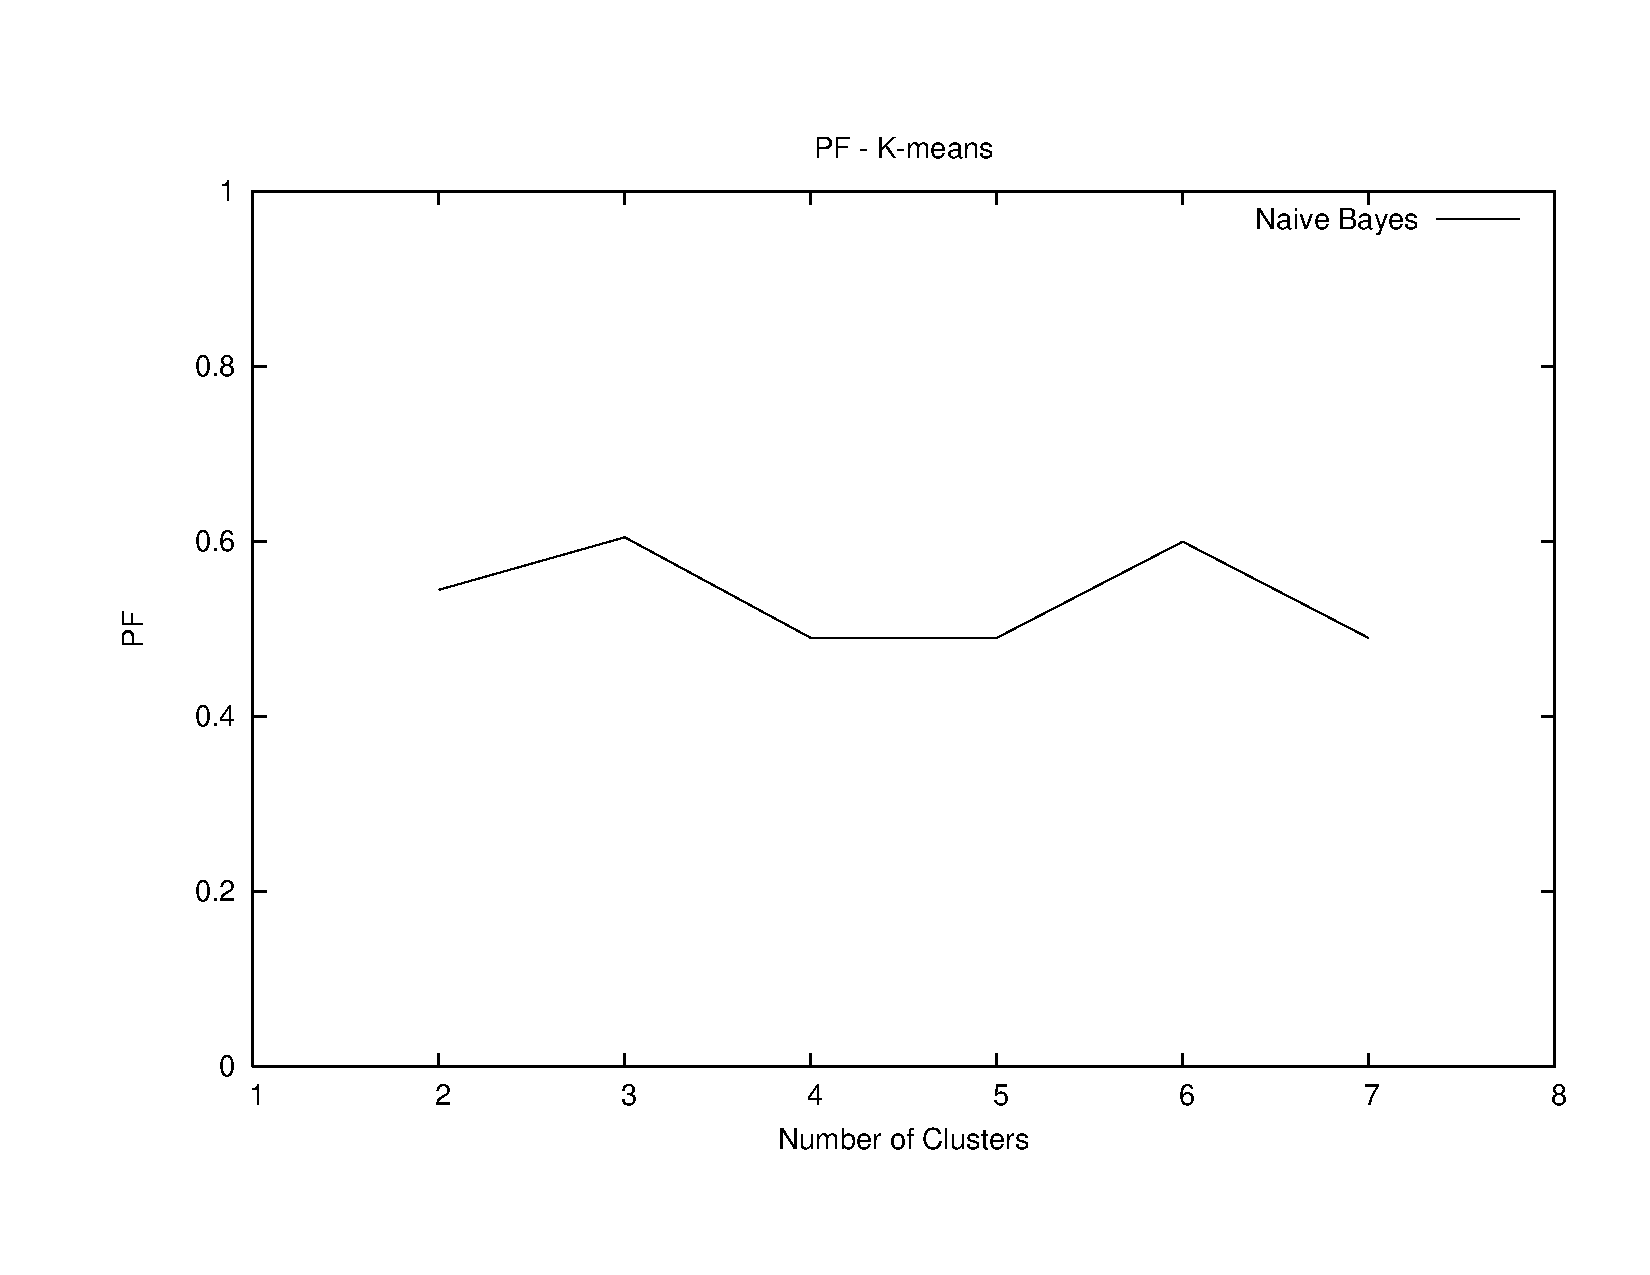
\includegraphics[width=3.5in]{no_disc_nb_cluster_pf.pdf}
  \end{center}

  \caption{\small Figure 2. PF: Naive-Bayes without discretization}
  \label{fig-label} \end{fig-label}
\end{figure}

PD and PF are ploted agains the number of clusters k. Without discretization Naive-Bayes does not perform well. PD is no higher than 60 \%. The number of clusters computed by k-means does not seem to influence the prediction probability however a relatively better PD are retrieved with 4, 5 and 7 clusters. This results also corresponds with \cite {dough95} which state that discretization influence Naive-Bayes performance.
\\
Applying InfoGain on discretize data outperforms the first learner. Data is discretized and InfoGain is used to extract the best n features (columns) from the data. Than Naive-Bayes is applyed on the closest cluster of each instance in the train set.Figure 3 and 4 show the PD and PF of this learner.

 \textbf
\begin
  \begin{center}
    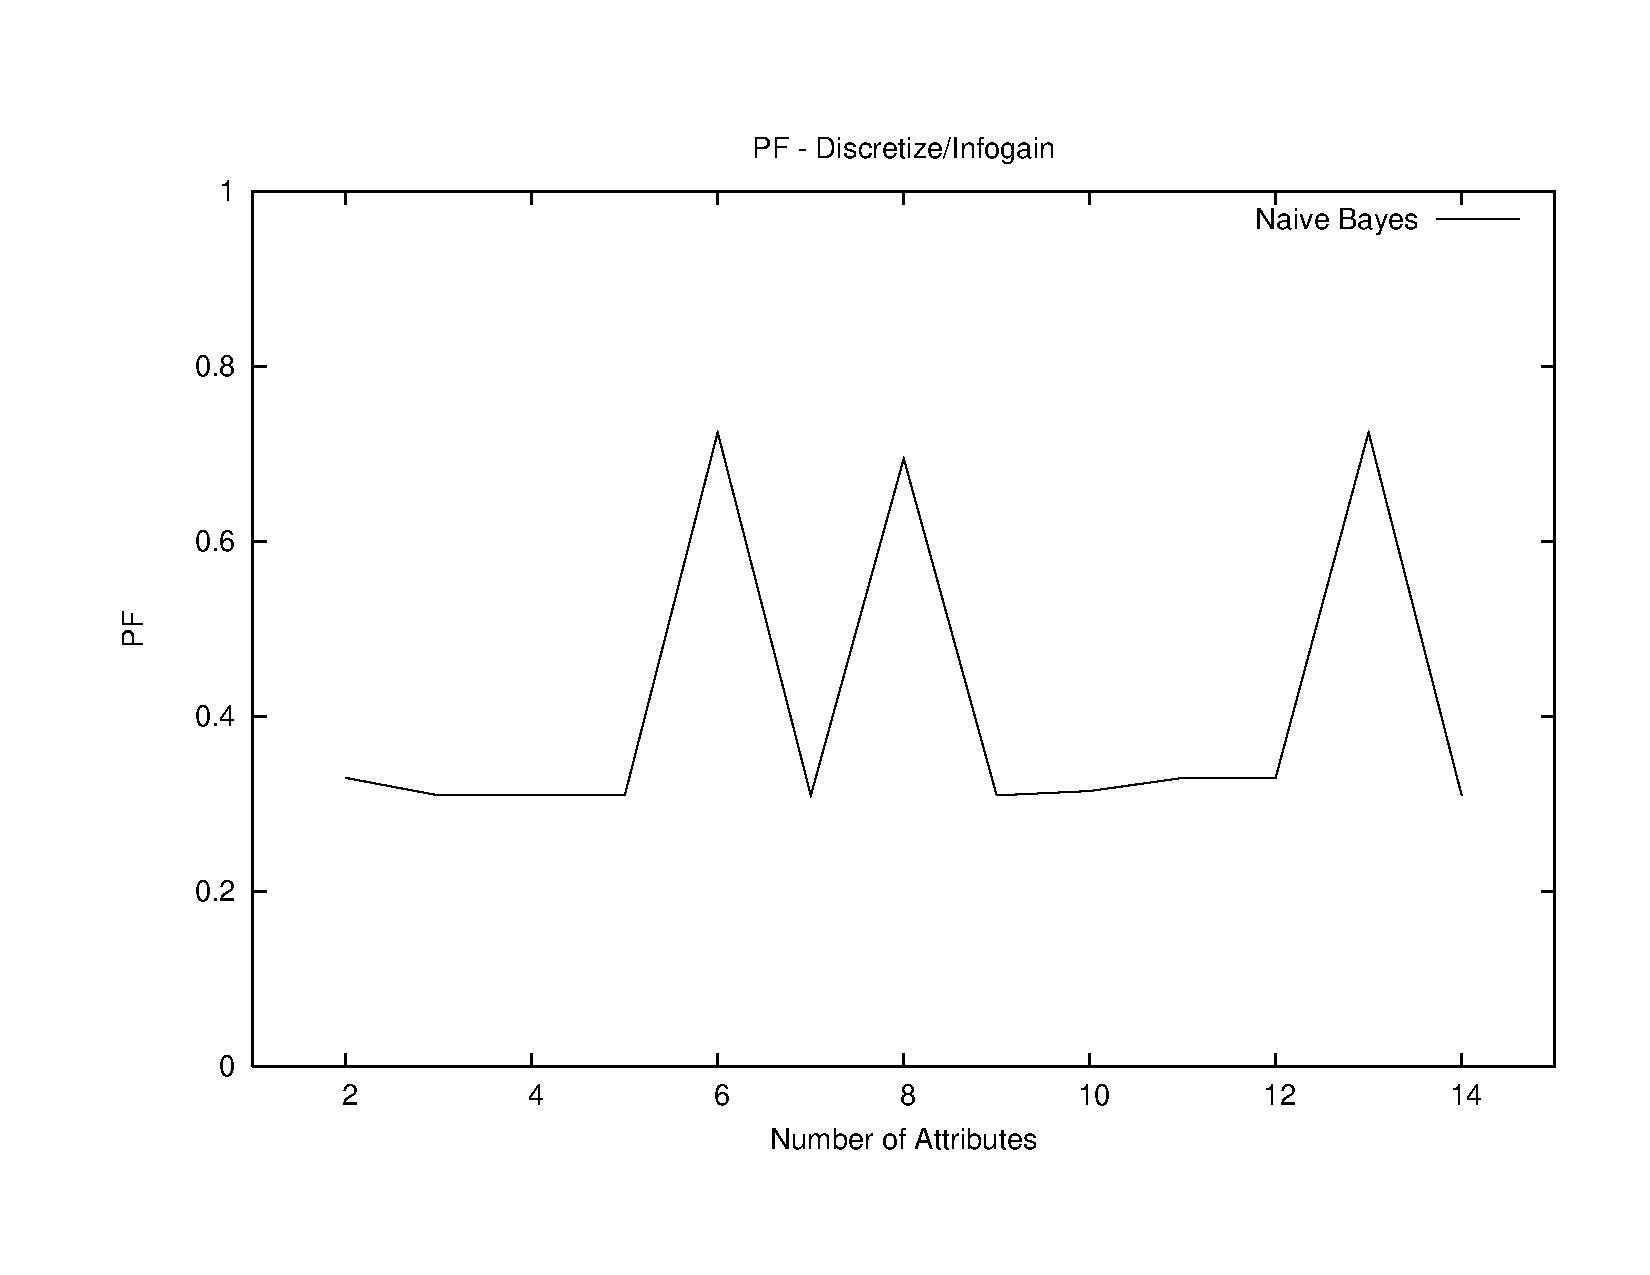
\includegraphics[width=3.5in]{disc_info_nb_pd.pdf}
  \end{center}

  \caption{\small Figure 3. PD: InfoGain and Naive-Bayes}
  \label{fig-label} \end{fig-label}
\end{figure}

\\
\\The second learner scores the highest values for PD when the number of attributes selected by InfoGain n is 6 & 8 and 13. The max PD values are close to 80 \%. In this case the advantage of discretizing the data and applying feature subset selection gives better results than applying the clustering on undiscretized data. 
\textbf
\begin
  \begin{center}
    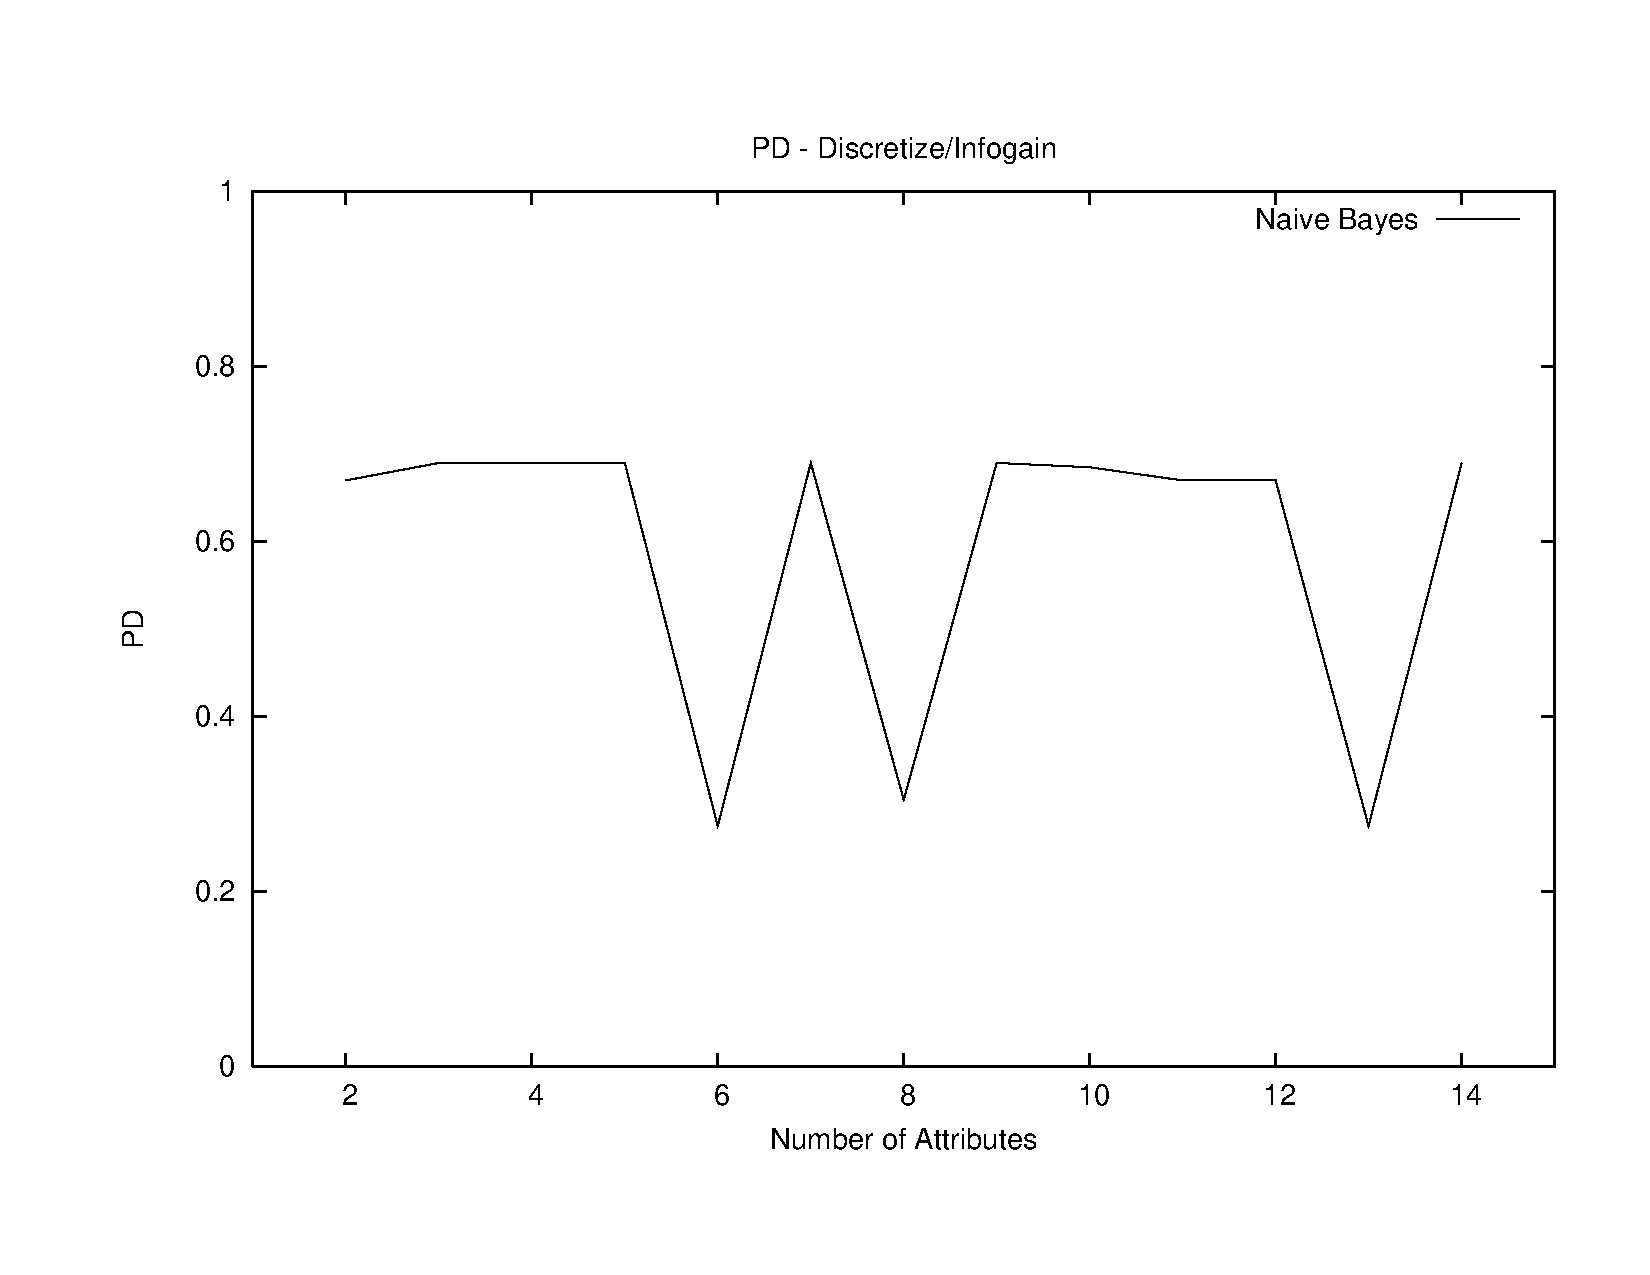
\includegraphics[width=3.5in]{disc_info_nb_pf.pdf}
  \end{center}
  \caption{\small Figure 4. PF InfoGain and Naive-Bayes}
  \label{fig-label} \end{fig-label}
\end{figure}

\\The third learner uses the information supplied by InfoGain to build a new data set containing only the features suggested by InfoGain. Discretization clustering is performed on the data using k-means and Naive-Bayes is trained on each cluster. This learner is exploring a combination of n-features and k-clusters in order to find the optimal solution. Figures 5 and 6 shows the PD and PF for the third learner.
 
\textbf
\begin
  \begin{center}
    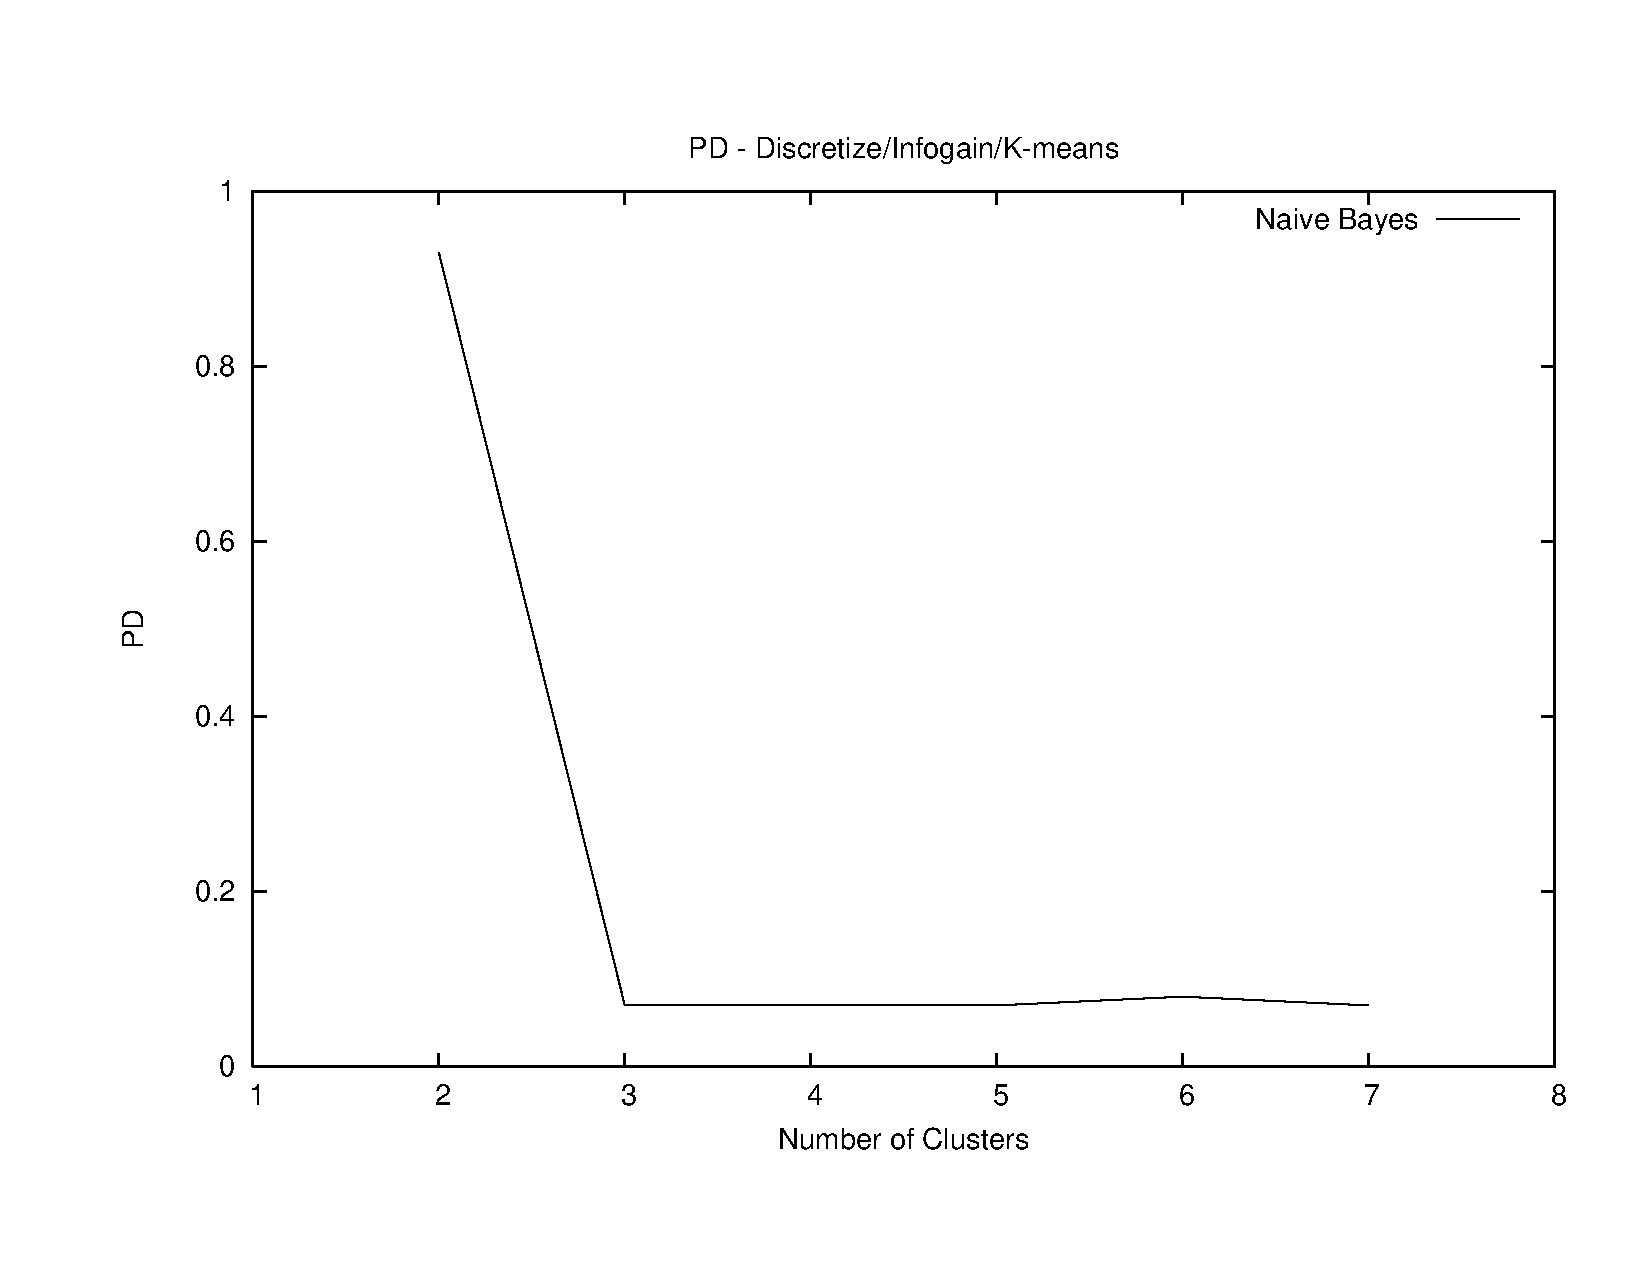
\includegraphics[width=3.5in]{disc_info_cluster_pd.pdf}
  \end{center}
  \caption{\small Figure 5. PD InfoGain/Clustering and Naive-Bayes}
  \label{fig-label} \end{fig-label}
\end{figure}

\textbf
\begin
  \begin{center}
    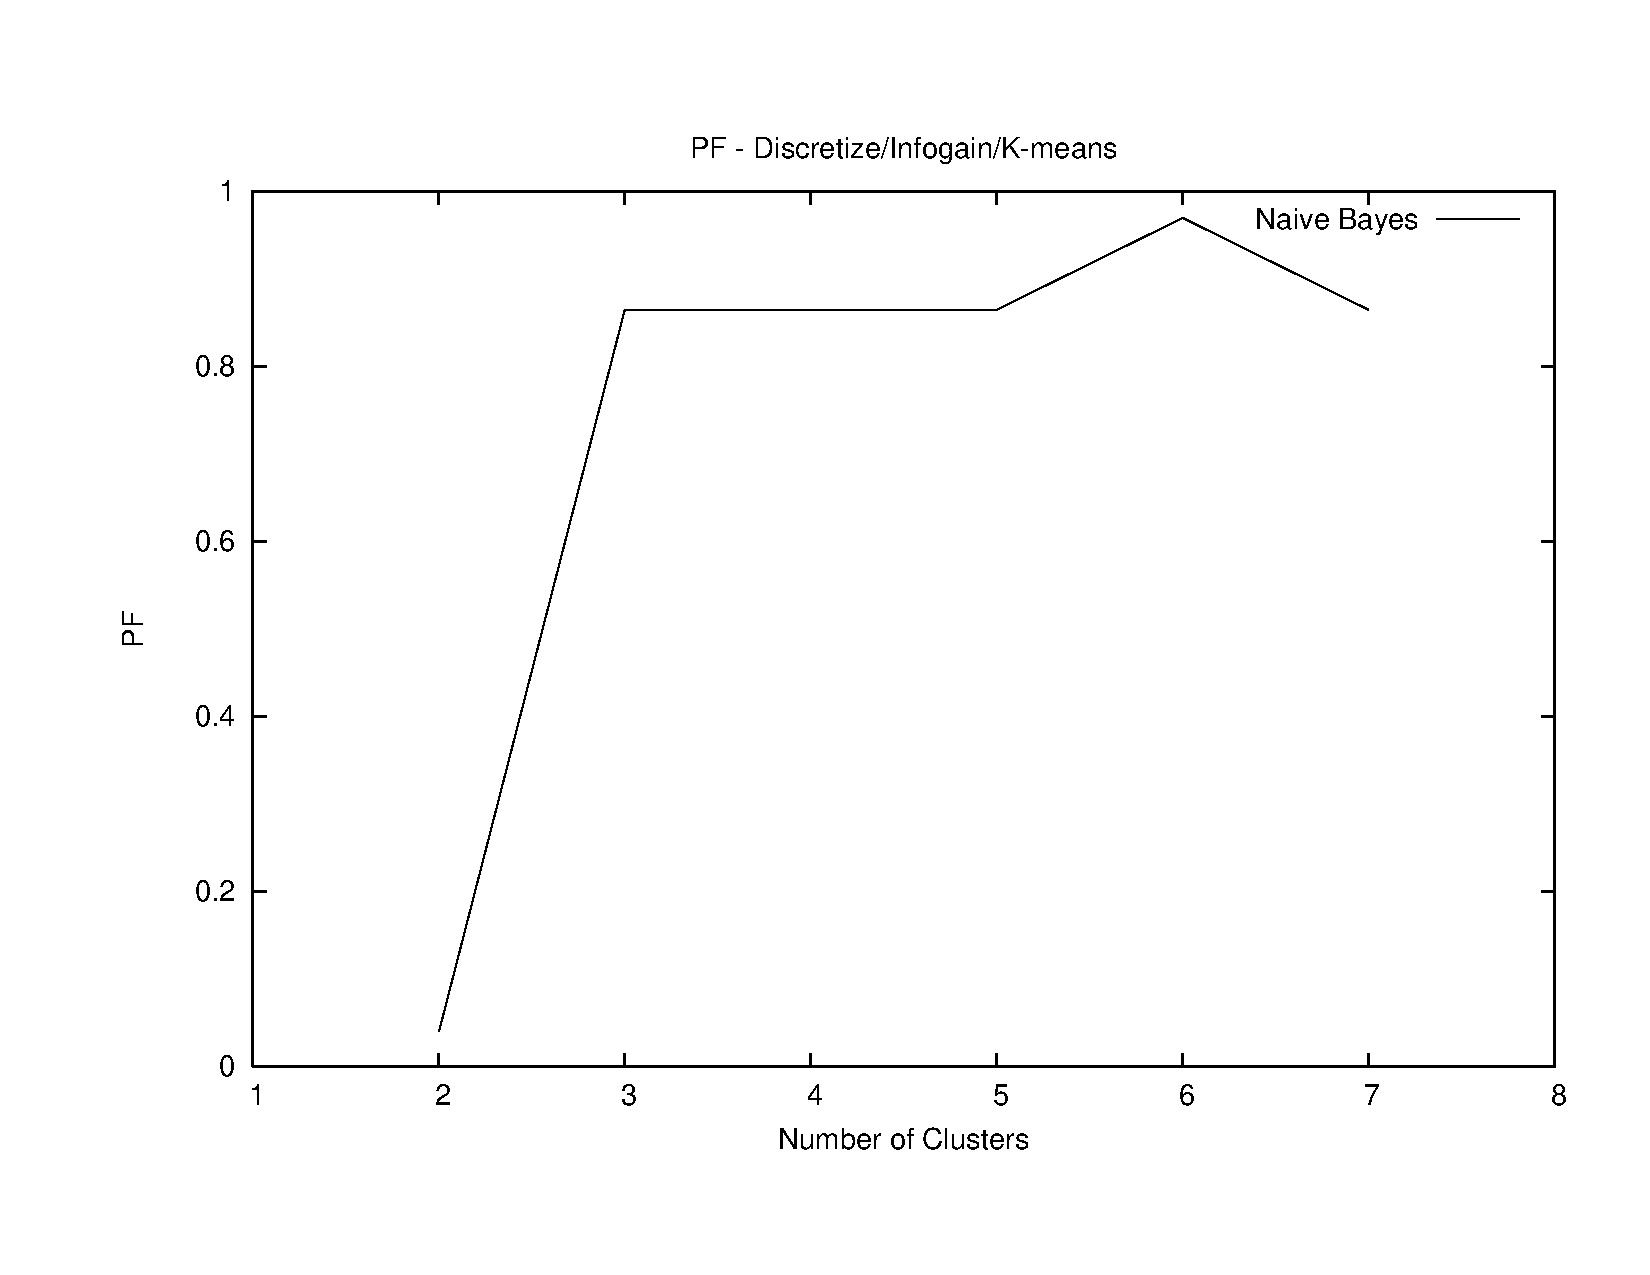
\includegraphics[width=3.5in]{disc_info_cluster_pf.pdf}
  \end{center}
  \caption{\small Figure 6. PF InfoGain/Clustering and Naive-Bayes}
  \label{fig-label} \end{fig-label}
\end{figure}

\\The figures show PD and PF plotted against k-number of clusters which varies from 2 to 7. The PD values increase sharply when 3 or more clusters are used. The PD remain unchanged as the number of clusters increases. The PD values are relatively high (more than 90 \%). These high results should be confirmed by performing further testing as to verify the validity of the learner. 
\\Table 1 Shows the top 13 attributes selected by InfoGain on each data set that was tested. 

\begin{table}
\centering
\caption{Frequency of Special Characters}
\begin{tabular}{|c|c|l|} \hline
Non-English or Math&Frequency&Comments\\ \hline
\O & 1 in 1,000& For Swedish names\\ \hline
$\pi$ & 1 in 5& Common in math\\ \hline
\$ & 4 in 5 & Used in business\\ \hline
$\Psi^2_1$ & 1 in 40,000& Unexplained usage\\
\hline\end{tabular}
\end{table}


\section{Related Work}
This project is inspired by the Cross-project Defect Prediction work conducted by Thomas Zimmerman et. al. who claimed that software defect prediction works well whenever there is sufficient data to train any models and that in the case where data is insufficient, cross-project defect prediction suffices\cite{zimmerman09}. In their experiment, they ran 622 cross-project predictions for 12 real-world applications including Microsoft's Internet Explorer and Mozilla Foundation's Firefox web browser, and their results indicated that simply using models from projects in the same domain or with the same process does not lead to accurate predictions. With respect to the experiments they conducted, they learned that Firefox could predict defects in Internet Explorer but not vice versa and they succumbed to the conclusion that this is so because Firefox has more files than Internet Explorer has binaries and that the probability of a software with more data is more likely to predict defects in software with relatively less amount of data or modules. 


\section{Conclusions}
Our study involves investigating a criteria for predicting default-prone modules in both large and small software systems. From the experiments performed on each of the data sets we obtained from NASA and SoftLab, we learned that within-company software defect prediction works when the data accumulated for prior versions of the software in question is available. The results from our self-test experiments validates this conclusion. In other words, creating train and test data from the same data set allows us to successfully build models for software defect prediction. This is especially feasible in cases where the company (whose datasets are being used in the experiment) has been around for years, for example NASA, Microsoft or the Mozilla Foundation; or older versions of its software have already been in use for years. The data generated from such older versions can be analyzed, learned on and used to build defect prediction models in order to predict defects in newer versions of the software.

Some researchers indicate that collecting data from case studies and subjecting it to isolated analysis is not enough because statistics on its own does not provide scientific explanations; and that ``we need compelling and sophisticated theories that have the power to explain the empirical observations''\cite{critique}. However, in our experiments, we ran 10 tests on 10 datasets, each time with a different number of nearest-neighbors and number of columns to be selected via infogain, and despite the fact that these experiments were conducted on randomly selected objects from the different data sets and resulted in inconsistencies in the accuracy of defect predictions, the average probability of detection was relatively high while the probability of false alarm was relatively low. Of course, these values were obtained after intensive analysis on the results from applying learners on our datasets which we pre-processed using a number of machine learning / data mining methods. These include: replacing numeric values N with log(N) if N > 0.0001 or just 0.0001 if otherwise; splitting the data set and building a train data from 90\% of the data and test data from the remaining 10\%; clustering the data by finding the k-th nearest neighbor of each instance, normalizing, discretizing and applying infogain on each data set.


\section{Future Work}
The experiments for this project were conducted using data obtained from NASA and SoftLab for this project simply because they are 2 complete different companies that operate and function in different ways. 
The National Aeronautics and Space Administration (NASA) is an agency of the United States government that undertakes the nation's projects related to space exploration and SoftLab on the other hand is a research laboratory of computer engineering in Turkey that conducts research on cost and effort estimation, defect estimation/prevention, value based software engineering and software process development. 

We believe that for better results and much better success rates at predicting software defects, regression algorithms could be applied to the datasets to model the data with the least error. That is, apply the learners to the datasets a number of times and discard arguments to algorithms such as k-nearest neighbor and infogain that germinated less desirable results. Also, the learning algorithms used could be altered to analyze additional data instances added to the data already learned on and determine whether the new data would be benefitial to predicting defects or not.
Furthermore, this work could be extended to exploit datasets that comprised of more than 2 classes (TRUE, FALSE) and with multiple class columns (at least 2).

Nonetheless, a number of other rule-based learners could be used rather than {\em NaiveBayes} as was used for this project. These include, but are not limited to, the {\em PRISM} algorithm which aims at inducing modular classification rules directly from the training set; {\em OneR}, {\em TwoR}, {\em RIPPER}, and even {\em HyperPipes}. Due to the constraint on time, we were unable to experiment on such learners but the outcome of applying each of them on the same datasets we used would be of great value to software engineers / data miners. 
Finally, because all the data sets we used were complete, the alrgorithms used in our experiments didn't account for missing values but in future implementations, this will have to be addressed since ignoring this problem can introduce bias into the models being evaluated and lead to inaccurate data mining conclusions \cite{missingdata}. This can easily be done by either ignoring the entire record, filling in with a global constant (not recommended since most data mining algorithms will regard it as a normal value), fill in with the attribute's mean or median, fill in with the most likely value (using regression, decisino trees, most similar records, etc) or using other attributes to predict the value of the missing data.


\section{The {\secit Body} of The Paper}
Typically, the body of a paper is organized
into a hierarchical structure, with numbered or unnumbered
headings for sections, subsections, sub-subsections, and even
smaller sections.  The command \texttt{{\char'134}section} that
precedes this paragraph is part of such a
hierarchy.\footnote{This is the second footnote.  It
starts a series of three footnotes that add nothing
informational, but just give an idea of how footnotes work
and look. It is a wordy one, just so you see
how a longish one plays out.} \LaTeX\ handles the numbering
and placement of these headings for you, when you use
the appropriate heading commands around the titles
of the headings.  If you want a sub-subsection or
smaller part to be unnumbered in your output, simply append an
asterisk to the command name.  Examples of both
numbered and unnumbered headings will appear throughout the
balance of this sample document.

Because the entire article is contained in
the \textbf{document} environment, you can indicate the
start of a new paragraph with a blank line in your
input file; that is why this sentence forms a separate paragraph.

\subsection{Type Changes and {\subsecit Special} Characters}
We have already seen several typeface changes in this sample.  You
can indicate italicized words or phrases in your text with
the command \texttt{{\char'134}textit}; emboldening with the
command \texttt{{\char'134}textbf}
and typewriter-style (for instance, for computer code) with
\texttt{{\char'134}texttt}.  But remember, you do not
have to indicate typestyle changes when such changes are
part of the \textit{structural} elements of your
article; for instance, the heading of this subsection will
be in a sans serif\footnote{A third footnote, here.
Let's make this a rather short one to
see how it looks.} typeface, but that is handled by the
document class file. Take care with the use
of\footnote{A fourth, and last, footnote.}
the curly braces in typeface changes; they mark
the beginning and end of
the text that is to be in the different typeface.

You can use whatever symbols, accented characters, or
non-English characters you need anywhere in your document;
you can find a complete list of what is
available in the \textit{\LaTeX\
User's Guide}\cite{Lamport:LaTeX}.

\subsection{Math Equations}
You may want to display math equations in three distinct styles:
inline, numbered or non-numbered display.  Each of
the three are discussed in the next sections.

\subsubsection{Inline (In-text) Equations}
A formula that appears in the running text is called an
inline or in-text formula.  It is produced by the
\textbf{math} environment, which can be
invoked with the usual \texttt{{\char'134}begin. . .{\char'134}end}
construction or with the short form \texttt{\$. . .\$}. You
can use any of the symbols and structures,
from $\alpha$ to $\omega$, available in
\LaTeX\cite{Lamport:LaTeX}; this section will simply show a
few examples of in-text equations in context. Notice how
this equation: \begin{math}\lim_{n\rightarrow \infty}x=0\end{math},
set here in in-line math style, looks slightly different when
set in display style.  (See next section).

\subsubsection{Display Equations}
A numbered display equation -- one set off by vertical space
from the text and centered horizontally -- is produced
by the \textbf{equation} environment. An unnumbered display
equation is produced by the \textbf{displaymath} environment.

Again, in either environment, you can use any of the symbols
and structures available in \LaTeX; this section will just
give a couple of examples of display equations in context.
First, consider the equation, shown as an inline equation above:
\begin{equation}\lim_{n\rightarrow \infty}x=0\end{equation}
Notice how it is formatted somewhat differently in
the \textbf{displaymath}
environment.  Now, we'll enter an unnumbered equation:
\begin{displaymath}\sum_{i=0}^{\infty} x + 1\end{displaymath}
and follow it with another numbered equation:
\begin{equation}\sum_{i=0}^{\infty}x_i=\int_{0}^{\pi+2} f\end{equation}
just to demonstrate \LaTeX's able handling of numbering.

\subsection{Citations}
Citations to articles \cite{bowman:reasoning,
clark:pct, braams:babel, herlihy:methodology},
conference proceedings \cite{clark:pct} or
books \cite{salas:calculus, Lamport:LaTeX} listed
in the Bibliography section of your
article will occur throughout the text of your article.
You should use BibTeX to automatically produce this bibliography;
you simply need to insert one of several citation commands with
a key of the item cited in the proper location in
the \texttt{.tex} file \cite{Lamport:LaTeX}.
The key is a short reference you invent to uniquely
identify each work; in this sample document, the key is
the first author's surname and a
word from the title.  This identifying key is included
with each item in the \texttt{.bib} file for your article.

The details of the construction of the \texttt{.bib} file
are beyond the scope of this sample document, but more
information can be found in the \textit{Author's Guide},
and exhaustive details in the \textit{\LaTeX\ User's
Guide}\cite{Lamport:LaTeX}.

This article shows only the plainest form
of the citation command, using \texttt{{\char'134}cite}.
This is what is stipulated in the SIGS style specifications.
No other citation format is endorsed or supported.

\subsection{Tables}
Because tables cannot be split across pages, the best
placement for them is typically the top of the page
nearest their initial cite.  To
ensure this proper ``floating'' placement of tables, use the
environment \textbf{table} to enclose the table's contents and
the table caption.  The contents of the table itself must go
in the \textbf{tabular} environment, to
be aligned properly in rows and columns, with the desired
horizontal and vertical rules.  Again, detailed instructions
on \textbf{tabular} material
is found in the \textit{\LaTeX\ User's Guide}.

Immediately following this sentence is the point at which
Table 1 is included in the input file; compare the
placement of the table here with the table in the printed
dvi output of this document.

\begin{table}
\centering
\caption{Frequency of Special Characters}
\begin{tabular}{|c|c|l|} \hline
Non-English or Math&Frequency&Comments\\ \hline
\O & 1 in 1,000& For Swedish names\\ \hline
$\pi$ & 1 in 5& Common in math\\ \hline
\$ & 4 in 5 & Used in business\\ \hline
$\Psi^2_1$ & 1 in 40,000& Unexplained usage\\
\hline\end{tabular}
\end{table}

To set a wider table, which takes up the whole width of
the page's live area, use the environment
\textbf{table*} to enclose the table's contents and
the table caption.  As with a single-column table, this wide
table will ``float" to a location deemed more desirable.
Immediately following this sentence is the point at which
Table 2 is included in the input file; again, it is
instructive to compare the placement of the
table here with the table in the printed dvi
output of this document.


\begin{table*}
\centering
\caption{Some Typical Commands}
\begin{tabular}{|c|c|l|} \hline
Command&A Number&Comments\\ \hline
\texttt{{\char'134}alignauthor} & 100& Author alignment\\ \hline
\texttt{{\char'134}numberofauthors}& 200& Author enumeration\\ \hline
\texttt{{\char'134}table}& 300 & For tables\\ \hline
\texttt{{\char'134}table*}& 400& For wider tables\\ \hline\end{tabular}
\end{table*}
% end the environment with {table*}, NOTE not {table}!

\subsection{Figures}
Like tables, figures cannot be split across pages; the
best placement for them
is typically the top or the bottom of the page nearest
their initial cite.  To ensure this proper ``floating'' placement
of figures, use the environment
\textbf{figure} to enclose the figure and its caption.

This sample document contains examples of \textbf{.eps}
and \textbf{.ps} files to be displayable with \LaTeX.  More
details on each of these is found in the \textit{Author's Guide}.

\begin{figure}
\centering
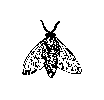
\epsfig{file=fly.eps}
\caption{A sample black and white graphic (.eps format).}
\end{figure}

\begin{figure}
\centering
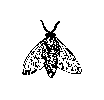
\epsfig{file=fly.eps, height=1in, width=1in}
\caption{A sample black and white graphic (.eps format)
that has been resized with the \texttt{epsfig} command.}
\end{figure}


As was the case with tables, you may want a figure
that spans two columns.  To do this, and still to
ensure proper ``floating'' placement of tables, use the environment
\textbf{figure*} to enclose the figure and its caption.
\begin{figure*}
\centering
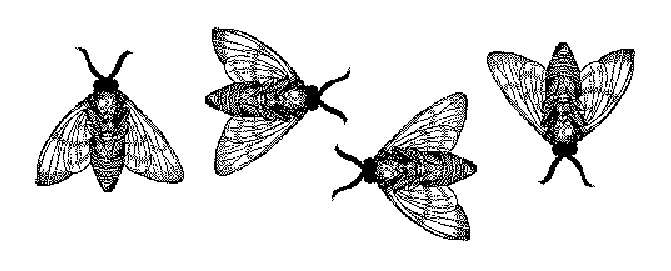
\epsfig{file=flies.eps}
\caption{A sample black and white graphic (.eps format)
that needs to span two columns of text.}
\end{figure*}
and don't forget to end the environment with
{figure*}, not {figure}!

Note that either {\textbf{.ps}} or {\textbf{.eps}} formats are
used; use
the \texttt{{\char'134}epsfig} or \texttt{{\char'134}psfig}
commands as appropriate for the different file types.

\begin{figure}
\centering
\psfig{file=rosette.ps, height=1in, width=1in,}
\caption{A sample black and white graphic (.ps format) that has
been resized with the \texttt{psfig} command.}
\vskip -6pt
\end{figure}

\subsection{Theorem-like Constructs}
Other common constructs that may occur in your article are
the forms for logical constructs like theorems, axioms,
corollaries and proofs.  There are
two forms, one produced by the
command \texttt{{\char'134}newtheorem} and the
other by the command \texttt{{\char'134}newdef}; perhaps
the clearest and easiest way to distinguish them is
to compare the two in the output of this sample document:

This uses the \textbf{theorem} environment, created by
the\linebreak\texttt{{\char'134}newtheorem} command:
\newtheorem{theorem}{Theorem}
\begin{theorem}
Let $f$ be continuous on $[a,b]$.  If $G$ is
an antiderivative for $f$ on $[a,b]$, then
\begin{displaymath}\int^b_af(t)dt = G(b) - G(a).\end{displaymath}
\end{theorem}

The other uses the \textbf{definition} environment, created
by the \texttt{{\char'134}newdef} command:
\newdef{definition}{Definition}
\begin{definition}
If $z$ is irrational, then by $e^z$ we mean the
unique number which has
logarithm $z$: \begin{displaymath}{\log e^z = z}\end{displaymath}
\end{definition}

Two lists of constructs that use one of these
forms is given in the
\textit{Author's  Guidelines}.
 
There is one other similar construct environment, which is
already set up
for you; i.e. you must \textit{not} use
a \texttt{{\char'134}newdef} command to
create it: the \textbf{proof} environment.  Here
is a example of its use:
\begin{proof}
Suppose on the contrary there exists a real number $L$ such that
\begin{displaymath}
\lim_{x\rightarrow\infty} \frac{f(x)}{g(x)} = L.
\end{displaymath}
Then
\begin{displaymath}
l=\lim_{x\rightarrow c} f(x)
= \lim_{x\rightarrow c}
\left[ g{x} \cdot \frac{f(x)}{g(x)} \right ]
= \lim_{x\rightarrow c} g(x) \cdot \lim_{x\rightarrow c}
\frac{f(x)}{g(x)} = 0\cdot L = 0,
\end{displaymath}
which contradicts our assumption that $l\neq 0$.
\end{proof}

Complete rules about using these environments and using the
two different creation commands are in the
\textit{Author's Guide}; please consult it for more
detailed instructions.  If you need to use another construct,
not listed therein, which you want to have the same
formatting as the Theorem
or the Definition\cite{salas:calculus} shown above,
use the \texttt{{\char'134}newtheorem} or the
\texttt{{\char'134}newdef} command,
respectively, to create it.

\subsection*{A {\secit Caveat} for the \TeX\ Expert}
Because you have just been given permission to
use the \texttt{{\char'134}newdef} command to create a
new form, you might think you can
use \TeX's \texttt{{\char'134}def} to create a
new command: \textit{Please refrain from doing this!}
Remember that your \LaTeX\ source code is primarily intended
to create camera-ready copy, but may be converted
to other forms -- e.g. HTML. If you inadvertently omit
some or all of the \texttt{{\char'134}def}s recompilation will
be, to say the least, problematic.
%\end{document}  % This is where a 'short' article might terminate

%ACKNOWLEDGMENTS are optional
\section{Acknowledgments}
This section is optional; it is a location for you
to acknowledge grants, funding, editing assistance and
what have you.  In the present case, for example, the
authors would like to thank Gerald Murray of ACM for
his help in codifying this \textit{Author's Guide}
and the \textbf{.cls} and \textbf{.tex} files that it describes.

%
% The following two commands are all you need in the
% initial runs of your .tex file to
% produce the bibliography for the citations in your paper.
\bibliographystyle{abbrv}
\bibliography{refs}  % sigproc.bib is the name of the Bibliography in this case
% You must have a proper ".bib" file
%  and remember to run:
% latex bibtex latex latex
% to resolve all references
%
% ACM needs 'a single self-contained file'!
%
%APPENDICES are optional
%\balancecolumns
\appendix
%Appendix A
\section{Headings in Appendices}
The rules about hierarchical headings discussed above for
the body of the article are different in the appendices.
In the \textbf{appendix} environment, the command
\textbf{section} is used to
indicate the start of each Appendix, with alphabetic order
designation (i.e. the first is A, the second B, etc.) and
a title (if you include one).  So, if you need
hierarchical structure
\textit{within} an Appendix, start with \textbf{subsection} as the
highest level. Here is an outline of the body of this
document in Appendix-appropriate form:
\subsection{Introduction}
\subsection{The Body of the Paper}
\subsubsection{Type Changes and  Special Characters}
\subsubsection{Math Equations}
\paragraph{Inline (In-text) Equations}
\paragraph{Display Equations}
\subsubsection{Citations}
\subsubsection{Tables}
\subsubsection{Figures}
\subsubsection{Theorem-like Constructs}
\subsubsection*{A Caveat for the \TeX\ Expert}
\subsection{Conclusions}
\subsection{Related Work}
\subsection{Future Work}
\subsection{Acknowledgments}
\subsection{Additional Authors}
This section is inserted by \LaTeX; you do not insert it.
You just add the names and information in the
\texttt{{\char'134}additionalauthors} command at the start
of the document.
\subsection{References}
Generated by bibtex from your ~.bib file.  Run latex,
then bibtex, then latex twice (to resolve references)
to create the ~.bbl file.  Insert that ~.bbl file into
the .tex source file and comment out
the command \texttt{{\char'134}thebibliography}.
% This next section command marks the start of
% Appendix B, and does not continue the present hierarchy
\section{More Help for the Hardy}
The sig-alternate.cls file itself is chock-full of succinct
and helpful comments.  If you consider yourself a moderately
experienced to expert user of \LaTeX, you may find reading
it useful but please remember not to change it.
%\balancecolumns % GM June 2007
% That's all folks!
\end{document}
